\chapter{SNOWGRID Clustering}
% - Vereilung der anströmrichtung\\
% - Rücksichtnahme der verschiedenhohen anzahl in den gruppen und breiten\\

% - anzahl der cluster anzahl --> mathematisch\\
% - anzhal subjektiv \\
% - Nordstau\\
% - Südstau\\
% - undefined\\
% - Abstimmung mit exper knowledge anpassung an gebiergskämmen\\


\section{Wind sector distribution}

The classification of the days with solid percipitation $\geq$ 5 mm in different windsectors is based on 
the Cost733cat \ref{sec:wetterlagenkat}. Their distribution pattern is displayed in figure 
\ref{fig:wind_distribution}. 

\begin{figure*}[ht]
    \centering
    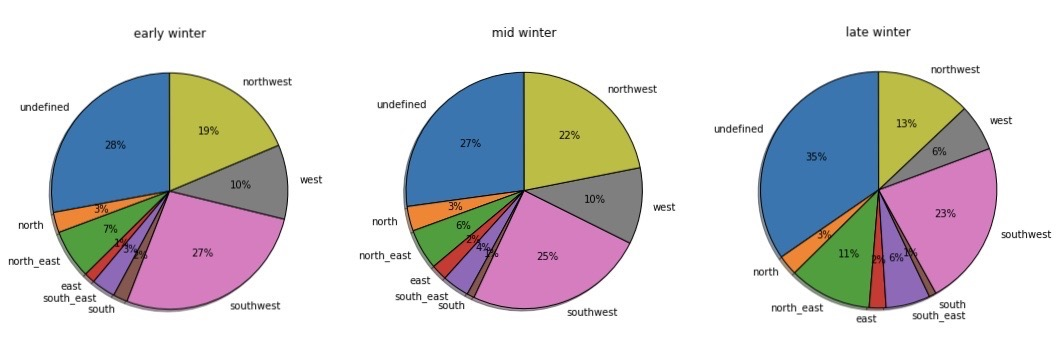
\includegraphics[width=\textwidth]{Figures/figures_snowgrid/windsector_seasons.jpg}
    \caption{Distribution of the days in windsectors within the winter seasons 
    from November 2011 till March 2021}
    \label{fig:wind_distribution}
\end{figure*}

\noindent The windsector with the most days counting is the sector 'undefined'- with changing windcontions 
throughout the day with round about 30 \%. For north blocking weather situations the biggest contrbution are 
coming from northwest for south blocking from southwest. Althoug of having a slim main windsector west it contributes 
8\% of the percipitation cases. Althogether it conclusive that it has more than 50 \% of the cases are having 
a west component, because of the location of alps on the northern hemisphere at 52 degree latitude. 

For further analysis of the typical percipitation habiits the cluster analysis should be applied diffrent typical
flows e.g:
\begin{itemize}
    \item north blocking (NW, N,NE)
    \item southblocking (SW, S, SE)
    \item west
    \item changing wind conditions
\end{itemize} 

\section{K-means: Number of Clusters}

\noindent For the k-means clustering the number of clusters must be predefind. Typically for the k-means clusting the 
elbow method is used to identify the optimum of number of groups. Increasing the number of clusters the
variation within a cluster will decrease. The optimum is reached when a further increasment does no lead to 
a significant increasement of the variation. Based on this five clusters should be 'mathematically' the best 
approach (Figure \ref{fig:5clusters}). Analsing the outerlines of the clusters we where not able to identify the 
patterns needed for this analysis which are not in line with expert knowledge of local observers. Therefore 
the number of clusters are increased until the boundarie-patterns show a higher familiar pattern. It has 
been subjektivly set to 15 clusters. (Figure \ref{fig:15clusters} )
\\
\\

- 5 warnregionen
- micro regions mehr bezug auf lokale rückmeldungen/probleme

\begin{minipage}{.5\textwidth}

    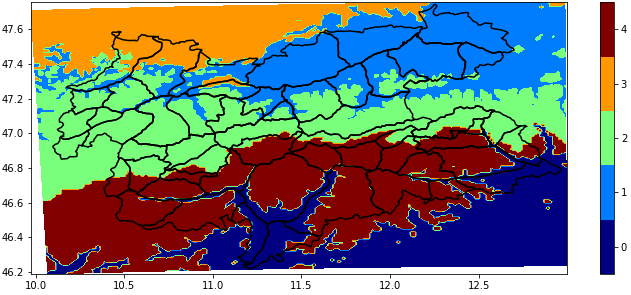
\includegraphics[width=\textwidth]{Figures/figures_snowgrid/clusters_analysis_north_5.png}
    \captionof{figure}{K-means clusters for daily snowcover height chance for  5 clusters  for 
    north blocking situations }
    \label{fig:5clusters}
    \end{minipage}
    \hfill
    \begin{minipage}{.5\linewidth}
    
    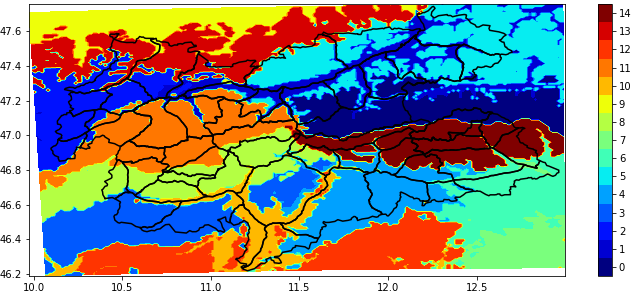
\includegraphics[width=\linewidth]{Figures/figures_snowgrid/clusters_analysis_north_15.png}
    \captionof{figure}{K-means clusters for daily snowcover height chance for  15 clusters for 
    north blocking situations}
    \label{fig:15clusters}
    \end{minipage}
\\





\section{Clusters: Wind dependency}

- verhalten der cluster im bezug auf wind \\
- warnregionen werden immer flexibel auf jeweilige wind situation angepasst --> micro regionen für spezifische situation
- welche Microregionen passen wo gibt es handlungsbedarf \\

\begin{figure}[ht] 
    \label{ fig7} 
    \begin{minipage}[b]{0.48\linewidth}
      \centering
      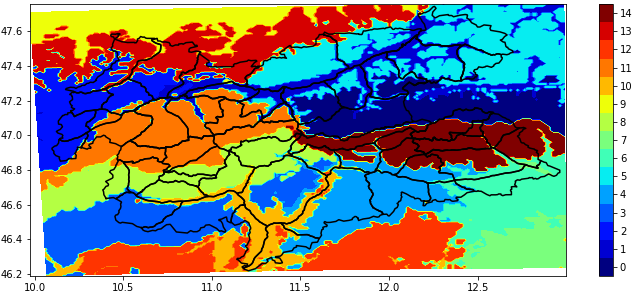
\includegraphics[width=0.9\linewidth]{Figures/figures_snowgrid/15_N_S_W_U/clusters_analysis_north15.png} 
      \caption{K-means clusters for daily snowcover height chance for  15 clusters for 
      north blocking situations} 
      \vspace{4ex}
      \hspace{4ex}
    \end{minipage}%%
    \begin{minipage}[b]{0.48\linewidth}
      \centering
      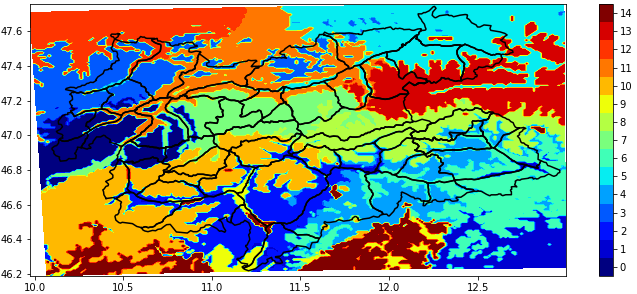
\includegraphics[width=0.9\linewidth]{Figures/figures_snowgrid/15_N_S_W_U/clusters_analysis_south15.png} 
      \caption{K-means clusters for daily snowcover height chance for  15 clusters for 
      south blocking situations} 
      \vspace{4ex}
      \hspace{4ex}
    \end{minipage} 
    \begin{minipage}[b]{0.48\linewidth}
      \centering
      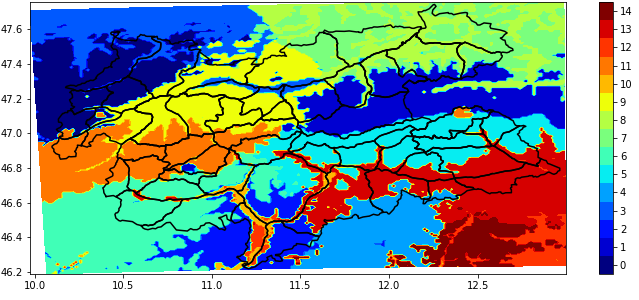
\includegraphics[width=0.9\linewidth]{Figures/figures_snowgrid/15_N_S_W_U/clusters_analysis_west_15.png} 
      \caption{K-means clusters for daily snowcover height chance for  15 clusters for
      west wind situations} 
      \vspace{4ex}
      \hspace{4ex}
    \end{minipage}%% 
    \begin{minipage}[b]{0.48\linewidth}
      \centering
      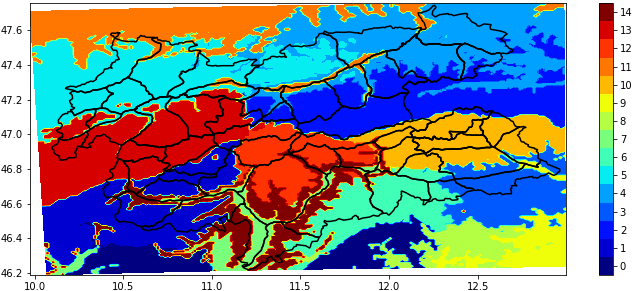
\includegraphics[width=0.9\linewidth]{Figures/figures_snowgrid/15_N_S_W_U/clusters_analysis_undefined_15.png} 
      \caption{K-means clusters for daily snowcover height chance for  15 clusters for changing wind conditions} 
      \vspace{4ex}
      \hspace{4ex}
    \end{minipage} 
  \end{figure}



\section{New Micro Regions}

\noindent To validate the builded clusters several local expertes where consulted to give the subjectiv percipitation
boundaries from their regions, without knowing the output from the clusteranalyis. The subjectiv approach
is overlayed by the cluster approach. Comparing both aproaches has led to adaptions in quite a few regions.
The final boundaries are fitted to alpine ridges, valleys and rivers. The final result is shown in fig . 


vergl experts zu cluster, neue grenzen definiert \\

\begin{figure}[ht] 
    \label{ fig7} 
    \begin{minipage}[b]{0.48\linewidth}
      \centering
      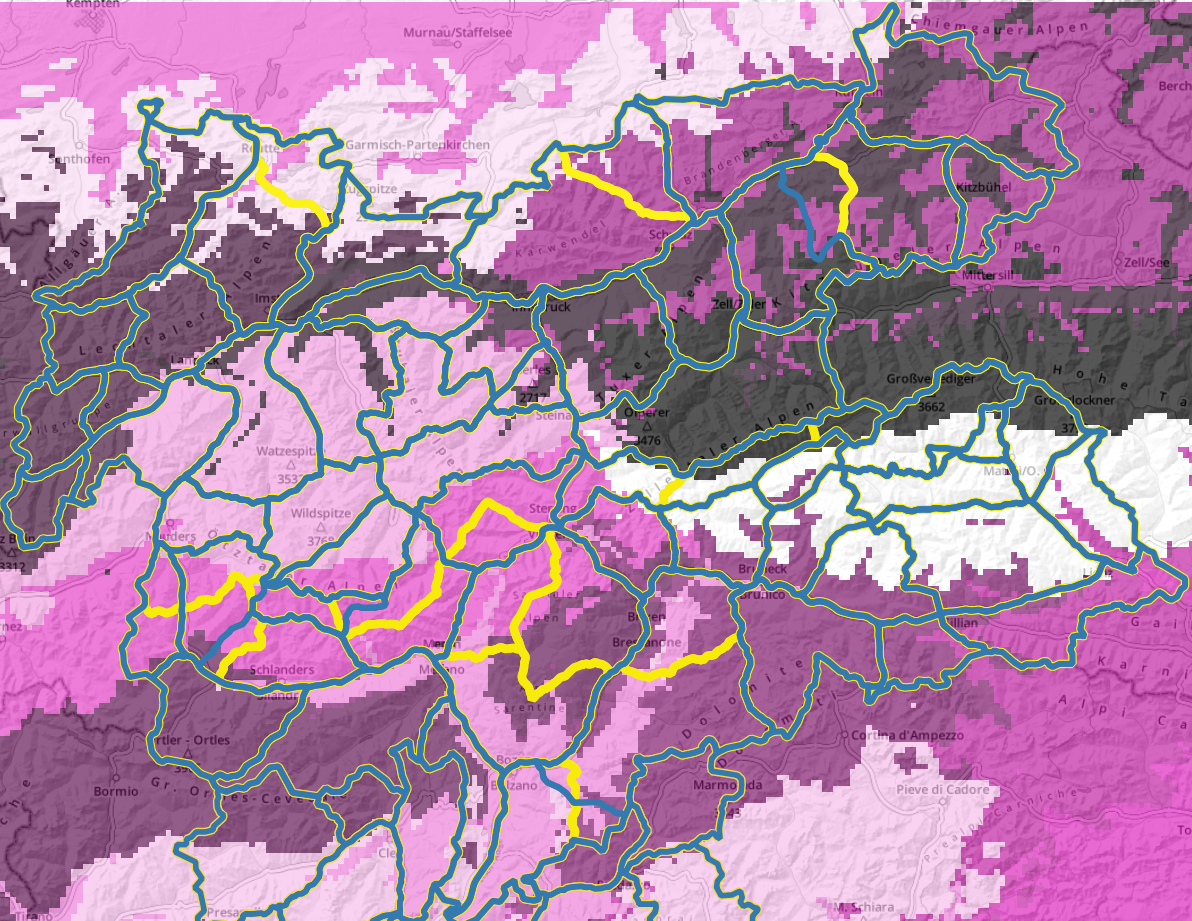
\includegraphics[width=0.9\linewidth]{Figures/figures_snowgrid/new_regions/new_regions_north_15.png} 
      \caption{North blocking: Comparison of k-means clustering and expert knowledge to preexisting micro-regions (blue) and
      new outerlines (green)} 
      \vspace{4ex}
      \hspace{4ex}
    \end{minipage}%%
    \begin{minipage}[b]{0.48\linewidth}
      \centering
      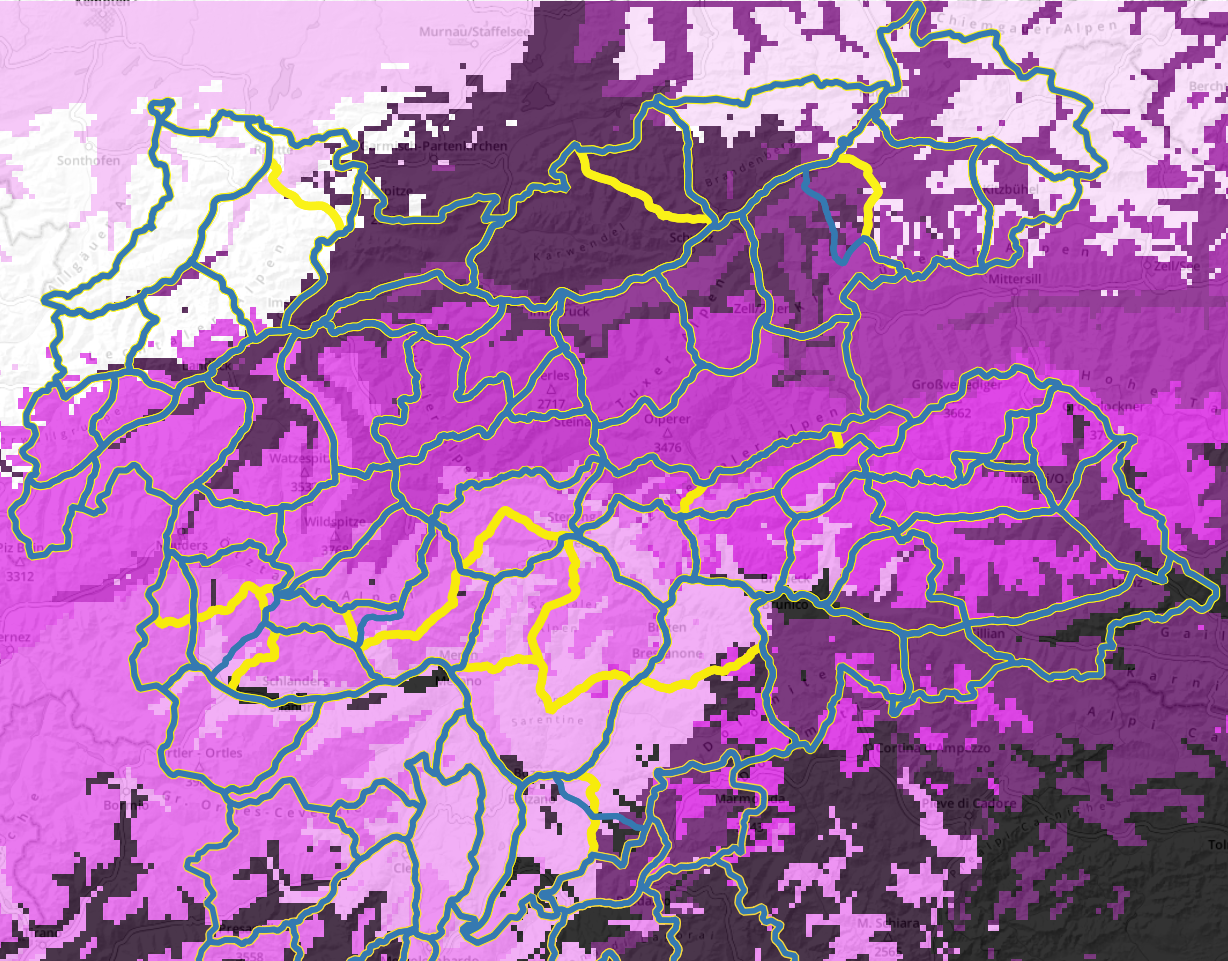
\includegraphics[width=0.9\linewidth]{Figures/figures_snowgrid/new_regions/new_regions_south_15.png} 
      \caption{South blocking: Comparison of k-means clustering and expert knowledge to preexisting micro-regions (blue) and
      new outerlines (green)} 
      \vspace{4ex}
      \hspace{4ex}
    \end{minipage} 
    \begin{minipage}[b]{0.48\linewidth}
      \centering
      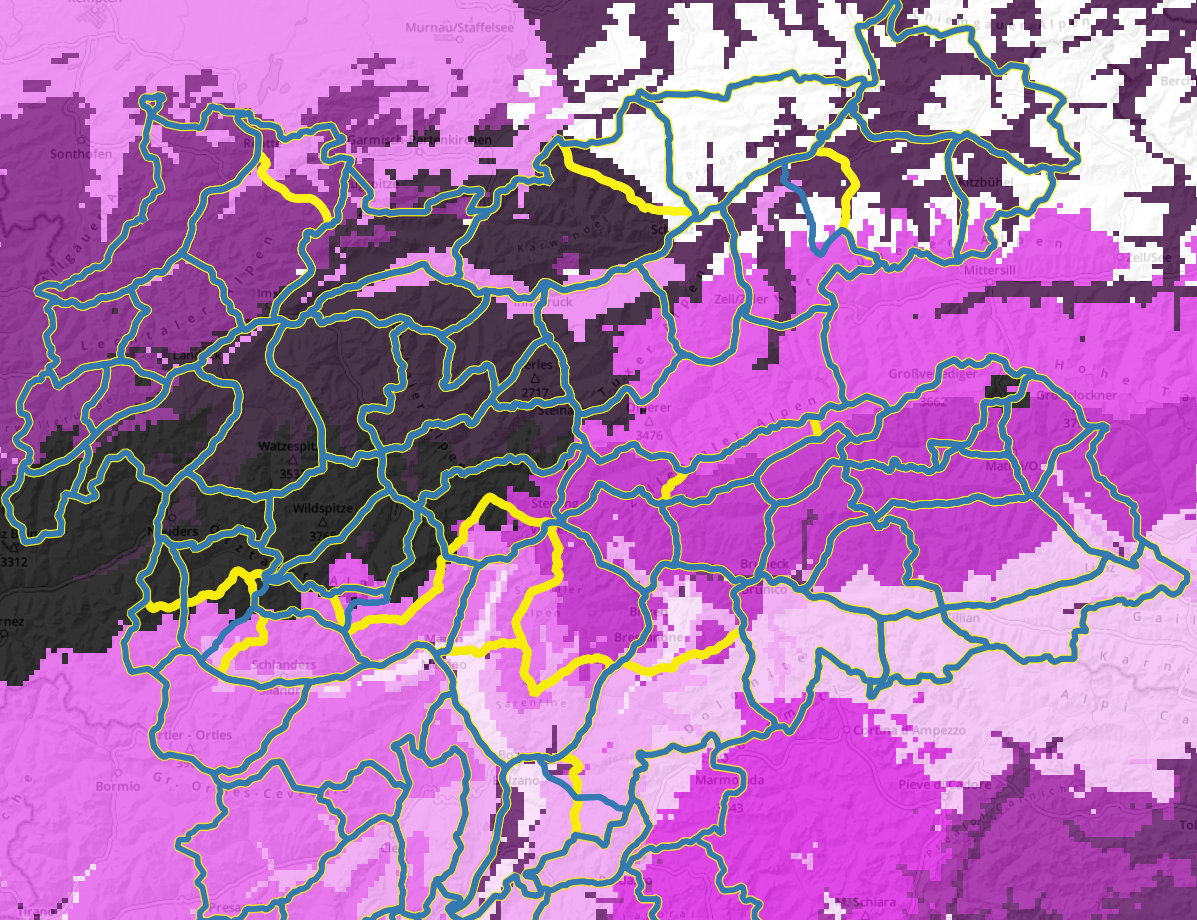
\includegraphics[width=0.9\linewidth]{Figures/figures_snowgrid/new_regions/new_regions_west_15.png} 
      \caption{West blocking: Comparison of k-means clustering and expert knowledge to preexisting micro-regions (blue) and
      new outerlines (green)} 
      \vspace{4ex}
      \hspace{4ex}
    \end{minipage}%% 
    \begin{minipage}[b]{0.48\linewidth}
      \centering
      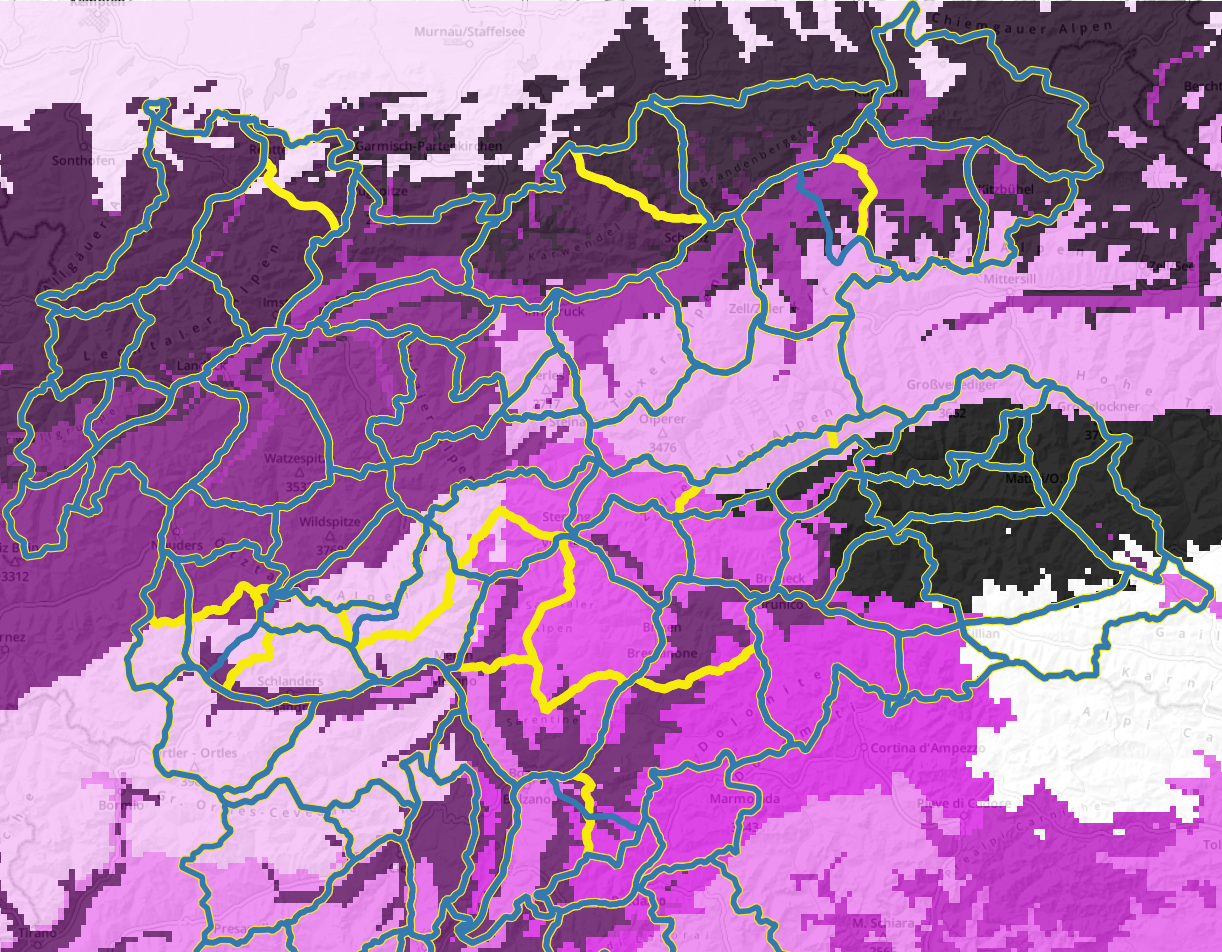
\includegraphics[width=0.9\linewidth]{Figures/figures_snowgrid/new_regions/new_regions_undef_15.png} 
      \caption{Changing wind conditions: Comparison of k-means clustering and expert knowledge to preexisting micro-regions (blue) and
      new outerlines (green)} 
      \vspace{4ex}
      \hspace{4ex}
    \end{minipage} 
  \end{figure}

